% Copyright (C) 2008, 2009, 2010, 2011, 2012, 2013, 2014 
% Bert Burgemeister
%
% Permission is granted to copy, distribute and/or modify this
% document under the terms of the GNU Free Documentation License,
% Version 1.2; with no Invariant Sections, no Front-Cover Texts and
% no Back-Cover Texts. For details see file COPYING.
%

\newcommand{\maintitle}{Cheatsheet By Hebi}
\newcommand{\AUTHOR}{Hebi Li}
%
%%%%%%%%%%%%%%%%%%
% pdf info
\newcommand{\SUBJECT}{Common\ Lisp}
\newcommand{\KEYWORDS}{{clqr cheatsheet lisp reference booklet}}
%
%%%%%%%%%%%%%%%%%%
% To be reset in paper-*.tex if there is plenty of room
\newcommand{\clearpagebeforeindex}{}
%
%
\documentclass[8pt,pagesize,twoside,footinclude=false,headinclude=false]{scrartcl}
%
%
%%%%%%%%%%%%%%%%%%

% outsourced page dimensions for letter paper
\setlength{\paperwidth}{4.25in}
\setlength{\paperheight}{11in}
%%\areaset[10mm]{8cm}{29cm}
\typearea[3mm]{20}
\renewcommand{\clearpagebeforeindex}{\clearpage}

% outsourced page dimensions for A4 paper
% \setlength{\paperwidth}{10.5cm}
% \setlength{\paperheight}{29.7cm}
% %%\areaset[10mm]{8cm}{29cm}
% \typearea[3mm]{20}
% \renewcommand{\clearpagebeforeindex}{\clearpage}



% outsourced hypertext colors
% for the printer-friendly version
\newcommand{\linkcolor}{black}
\newcommand{\urlcolor}{black}
\newcommand{\bookmarks}{false}
\newcommand{\pdfpagelayout}{SinglePage}
% outsourced hypertext colors
% for the screen-only version
% \newcommand{\linkcolor}{Fuchsia}
% \newcommand{\urlcolor}{MidnightBlue}
% \newcommand{\bookmarks}{true}
% \newcommand{\pdfpagelayout}{TwoColumnLeft}

%%%%%%%%%%%%%%%%%%
%

\usepackage{tikz}
\usetikzlibrary{shapes.multipart}
\usetikzlibrary{patterns}
\usetikzlibrary{positioning,fit,calc}
\usetikzlibrary{decorations.pathmorphing}
\usetikzlibrary{decorations.pathreplacing}
\usetikzlibrary{quotes}
\usetikzlibrary{graphs}
\usetikzlibrary{arrows.meta}



\usepackage{amsmath}
\usepackage{amsfonts}
\usepackage{amssymb}

\usepackage[mathcal]{euscript}


\usepackage{rotating}
\usepackage{graphicx}
\usepackage{multicol}
\usepackage{textcase}
% (HEBI: cannot load color again because perhaps the tikz package loaded it)
% \usepackage[usenames,dvips]{color}
\usepackage{suffix}
\usepackage{makeidx}
% (HEBI: and these colors needs color package, so move tikz above)
\definecolor{frontcovergray}{gray}{.85}
\definecolor{backcovergray}{gray}{.9}
\usepackage[pagestyles]{titlesec}
\usepackage{titletoc}


% my packages
\usepackage{listings}
\usepackage{textcomp}
\usepackage[inline]{enumitem}
\usepackage{courier}
\usepackage{indentfirst} % indent first paragraph after section
\usepackage{ulem}




%
%%%%%%%%%%%%%%%%%%
% Two font alternatives:
% (A) All (except cover pages) Computer Modern --
%     everything comes from the same sound root; gets about 5% longer
%     than alternative (B) 
\usepackage{type1cm}
\usepackage{exscale}
%%%%%%%%%%%%%%%%%%
% (B) Times mixed with Helvetica --
%     different sources; need scaling as they don't even agree in
%     their concept of height
%\usepackage{mathptmx}
%\usepackage[scaled]{helvet}
%%%%%%%%%%%%%%%%%%
%

% should remain last usepackage:
\usepackage%
    [breaklinks,linktocpage,colorlinks,%
      bookmarksnumbered,bookmarks=\bookmarks,%
      linkcolor=\linkcolor,urlcolor=\urlcolor,%
      pdfpagelayout=\pdfpagelayout,%
      pdftitle=\maintitle,pdfauthor=\AUTHOR,%
      pdfsubject=\SUBJECT,pdfkeywords=\KEYWORDS]%
    {hyperref}
%
\makeindex
\titleformat{\section}{\sffamily\mdseries\slshape}
            {\huge\thesection}{.7em}{\huge}[{\titlerule[0.25pt]}]
            
\titleformat{\subsection}{\sffamily\mdseries\slshape}
            {\Large\thesubsection}{.7em}{\Large}[{\titlerule[0.25pt]}]

% Kill toc header as we want it to span columns
\deftocheading{toc}{}

\titlecontents{section}%
[1.5em]%
{\vspace{.5em plus 1em minus .2em}\sffamily\bfseries\upshape\filright}%
{\contentslabel{1.5em}}%
{\hspace*{3em}}%
{\hfill\contentspage\vspace{.1em}}%

\titlecontents{subsection}%
[4em]%
{\sffamily\mdseries\upshape\filright}%
{\contentslabel{2.5em}}%
{\hspace*{5.5em}}%
{\hspace{.5ex plus .5ex minus .3ex}\titlerule*[1em]{.}\contentspage}%





%% my settings
\lstset{upquote=true} % for back quote, need textcomp
\lstset{basicstyle=\ttfamily\small,breaklines=true}
% \lstset{frame=b}
% \lstset{float,floatplacement=H,captionpos=b}
% \lstset{numbers=left}
% \lstset{language=C}
\lstset{showstringspaces=false}
% \lstset{framextopmargin=10pt}
% \lstset{framextopmargin=50pt,frame=t}
% \lstset{float=htb,language=C,frame=single, basicstyle=\small, stringstyle=\ttfamily}
% \lstset{escapeinside={(*@}{@*)}}

\setlist[description]{nosep
  ,style=sameline,leftmargin=3cm
  ,font=\ttfamily
}
\setlist[itemize]{nosep}
\setlist[enumerate]{nosep}

\newlist{inlineitemize}{itemize*}{1}
\newlist{inlineenumerate}{enumerate*}{1}
\newlist{inlinedescription}{description*}{1}

% I have to have the setlist* to make it work
% and this only works for enumerate
\setlist*[inlineenumerate,1]{label=(\roman*)}

\newcommand{\NT}[1]{\textnormal{\texttt{#1}}}

              
% \input{clqr.macros}
%
\begin{document}

\newlength{\titlepagewidth}
\setlength{\titlepagewidth}{8cm}
%%%%%%%%%%%%%%%%%%%%%%%%%%%%%%%%%%%%%%%%%%%%%%%%%%
%% Front Cover
%%%%%%%%%%%%%%%%%%%%%%%%%%%%%%%%%%%%%%%%%%%%%%%%%%
\begin{titlepage}
  \renewcommand{\rmdefault}{ptm} %% Always times fonts on title
  \advance\oddsidemargin by 1.5mm
  \vspace*{15mm}
  \begin{center}
    \begin{minipage}{\titlepagewidth}
      \begin{center}
        \rmfamily\mdseries\itshape\fontsize{20}{0}\selectfont
        An Open Cheat Sheet to be precise and consistent\index{CLQR}\\
      \end{center}
    \end{minipage}
    \vfill
    \begin{minipage}{\titlepagewidth}
      \begin{center}
        \rmfamily\mdseries\itshape%
        \fontsize{200}{0}\selectfont{\color{frontcovergray}OS\/}\\
      \end{center}
    \end{minipage}
    \vfill
    \begin{minipage}{\titlepagewidth}
      \rmfamily\mdseries\itshape\fontsize{36}{0}\selectfont
      \hfill Open\/\\[2mm]
      \rmfamily\mdseries\upshape\fontsize{107}{0}\selectfont
      \rule[0mm]{\textwidth}{1.5mm}\\
      Sheat\\[1mm]
      \rule[15mm]{\textwidth}{1.5mm}\\
      % \rule[15mm]{5.5cm}{1.5mm}\hfill\rule[15mm]{1.77cm}{1.5mm}
    \end{minipage}\\
    \begin{minipage}{\titlepagewidth}
      \rmfamily\mdseries\upshape\fontsize{14}{0}\selectfont
      \AUTHOR
      \vspace*{4mm}
    \end{minipage}
  \end{center}

\end{titlepage}

%%%%%%%%%%%%%%%%%%%%%%%%%%%%%%%%%%%%%%%%%%%%%%%%%%
% TOC
%%%%%%%%%%%%%%%%%%%%%%%%%%%%%%%%%%%%%%%%%%%%%%%%%%
\section*{\contentsname}
\vspace{-3ex}
{%
  \setlength{\columnsep}{1.5em}%
  \begin{multicols}{2}
    \tableofcontents
  \end{multicols}%
}
%%%%%%%%%%%%%%%%%%%%%%%%%%%%%%%%%%%%%%%%%%%%%%%%%%
\vfill
%%%%%%%%%%%%%%%%%%%%%%%%%%%%%%%%%%%%%%%%%%%%%%%%%%
%%%%%%%%%%%%%%%%%%%%%%%%%%%%%%%%%%%%%%%%%%%%%%%%%%
%%%  CONTENT STARTS HERE  %%%%%%%%%%%%%%%%%%%%%%%%
%%%%%%%%%%%%%%%%%%%%%%%%%%%%%%%%%%%%%%%%%%%%%%%%%%

\clearpage

% I use many descriptions, reduce the sep spacing
% \global\setlength{\itemsep}{-5pt}

\section{Emacs}

\subsection{general}
\begin{description}
\item [list-face-displays]
\item [fill-region]
\item [list-package] open the \texttt{*package*} buffer, \texttt{Ux}
  to update all.
\item [helm-etags-select]
\end{description}

\subsection{help}
\begin{description}
\item [describe-key-briefly] \texttt{C-h c} command name for a key
  stroke.
\item [where-is] \texttt{C-h w}, shortcut for a command
\item [info] \texttt{C-h i} open the built-in info reader.
\item [view-echo-area-messages]
\end{description}

\subsection{Dired}
\begin{description}
\item [dired-next-subdir]
\item [dired-prev-subdir]
\item [dired-tree-up]
\item [dired-tree-down]
\end{description}

\subsection{window}
\begin{description}
\item [balance-window]
\item [toggle-window-split]
\end{description}

\subsection{file}
\begin{description}
\item [revert-buffer] Reload file on disk
\item [recover-file] recover from \texttt{\#xxx\#} file.
\item [read-only-mode] disable it to edit read only files
\end{description}

\subsection{edit}

\begin{description}
\item [replace-rectangle]
\item [upcase-word]
\item [downcase-word]
\item [transpose-words]
\item [transpose-lines]
\item [C-q xxx] insert a control sequence
\item [capitalize-word]
\item [fill-paragraph]
\item [fill-region]
\item [auto-fill-mode]
\item [zap-to-char]
\item [zap-up-to-char]
\item [ispell] check spell 
\item [flycheck] check on-the-fly
\end{description}

\subsection{programming}

\begin{description}
\item [checkdoc] check the warnings in doc string
\item [C-x C-e] evaluate
\item [C-u C-x C-e] evaluate and insert result
\item [C-M-a] move to the beginning of defun
\item [C-M-e] move to the end of defun
\item [C-M-h] mark defun
\item [C-M-f] move forward a sexp
\item [C-M-b] move backward a sexp
\item [C-M-k] kill a sexp
\item [C-M-t] transpose expressions
\item [C-M-<SPC>] mark following sexp
\item [C-M-n] move to the next sexp
\item [C-M-p] move to the previous sexp
\item [C-M-u] move up parenthesis
\item [C-M-d] move down parenthesis
\item [C-M-x] evaluate defun
\item [forward-sexp] forward semantic block
\item [backward-sexp]
\item [org-forward-heading-same-level] =C-c C-f=
\item [org-backword-heading-same-level] =C-c C-b=
\end{description}

\subsection{Marking}
\begin{description}
\item [exhange-point-and-mark]
\item [mark-word]
\item [mark-sexp]
\item [mark-paragraph]
\item [mark-defun]
\item [mark-page]
\item [mark-whole-buffer]
\item [set-mark-command] C-SPC, set mark, and activate it
\item [C-SPC C-SPC] set mark, but not activate it.
\item [C-u C-SPC] pop to previous mark in mark ring. current is stored
  at the end of mark ring(rotating)
\item [pop-global-mark] will store both position and buffer
\item [set the mark] \texttt{C-SPC C-SPC}, \texttt{C-w}, search
\end{description}

\subsection{Register}
\begin{description}
\item [point-to-register] save ppposition in a register
\item [jump-to-register]
\item [jump-to-register] the register can store a file
\item [copy-to-register]
\item [insert-register]
\end{description}


\subsection{Key Map}
To configure a specific key map.  Note that the =global-set-key= will
\textit{not} overwrite a specific key map, because the specific one has a
higher priority.

\begin{lstlisting}[language=lisp]
  (define-key org-mode-map (kbd "C-j")
    (lambda()
      (interactive)
      (join-line -1)))
\end{lstlisting}

\subsection{Variables}
\paragraph{File Local Variable}
Emacs looks for the following line on first line or second line if
first line is shebang. \texttt{mode} defines the major mode for this
file, while unlimited number of variables follows, separated by
\texttt{;}.

\begin{lstlisting}
-*- mode: Lisp; fill-column: 75; comment-column: 50; -*-=
\end{lstlisting}


A second way to specify file local variable is to have a ``local
variables list'' near the end of the file (no more than 3000
characters from the end of the file).  The =LocalXXX Variables:= and
=XXXEnd:= will be matched literally, so literal that I have to add XXX
to these $\ldots$
\begin{lstlisting}
This     /* Local XXX Variables:  */
Is       /* mode: c           */
Garbage  /* comment-column: 0 */
AuCTex   TeX-master: "cheatsheet"
Data     /* XXXEnd:           */
\end{lstlisting}

\paragraph{Directory Local Variable}
Put \texttt{.dir-locals.el} at the root directory, and it will be in
effect for all the files under that directory, recursively.  It should
be an associate list, the car can be either a mode name (or \texttt{nil}
applies to all modes) indicating the variables are for that mode, or a
sub-directory name to apply only in that directory.
\begin{lstlisting}[language=lisp]
((nil . ((indent-tabs-mode . t)
         (fill-column . 80)))
 (c-mode . ((c-file-style . "BSD")
            (subdirs . nil)))
 ("src/imported"
  . ((nil . ((change-log-default-name
              . "ChangeLog.local"))))))
\end{lstlisting}


\subsection{Info}
Info is a document system.  It is closely bundled with emacs, so I put
it here.  To install some new info document in the system, issue the
following commands (using =gnu-c-manual= as an example):

\begin{lstlisting}
# download the gnu-c-manual code
make gnu-c-manual.info
mv gnu-c-manual.info /usr/local/share/info
cd /usr/local/share/info
sudo install-info --info-file=gnu-c-manual.info --info-dir=.
\end{lstlisting}

\subsubsection{Info Operations}

\begin{description}
\item [SPC] page down, can cross node
\item [BACKSPACE] page up, can cross node
\item [M-n] \texttt{clone-buffer}, open a new info buffer
\item [n] next node on same level
\item [p] previous
\item [{[}] next node regardless of level
\item [{]}] previous
\item [u] up node
\item [l] back
\item [r] forward
\item [m] ~Info-menu~, convenient for search node title
\item [s] TODO search  a text in the whole info file
\item [i] TODO search indices only
\end{description}


\subsection{YASnippet}
Put this into latex-mode directory as a file named ``desc'', and run \texttt{yas-reload-all}.
\begin{lstlisting}[language=tex]
# -*- mode: snippet -*-
# name: desciption
# key: desc
# --
\begin{description}
$1
\end{description}
$2
\end{lstlisting}
% \subsection{Babel}
% How to write a \texttt{ob-xxx.el} file?

% \begin{enumerate}
% \item search org-mode babel, you will get a link:
%   http://orgmode.org/worg/org-contrib/babel/
% \item In this link, there's a "languages"
%   link. http://orgmode.org/worg/org-contrib/babel/languages.html
% \item Under "Develop support for new languages" section, there's link
%   to ob-template.el:
%   http://orgmode.org/w/worg.git/blob/HEAD:/org-contrib/babel/ob-template.el
% \item follow instruction to modify it.
% \end{enumerate}
% some good example to look at: ob-plantuml.el, ob-C.el

%%% Local Variables:
%%% TeX-master: "cheatsheet"
%%% End:

\clearpage
\section{Elisp}
\subsection{Concepts}

\subsubsection{Quote}
\begin{tabular}{@{}ll@{}}
  \lstinline!'! & read without evaluate \\
  \lstinline!`! & same as \lstinline!'! except it can partially evaluate.\\
  \lstinline!,! & evaluate inside back quote\\
  \lstinline!,@! & evaluate and splice the resulting list inside back quote.
\end{tabular}

\subsubsection{Symbol}
Three special forms define symbols: \texttt{defvar}, \texttt{defun}, and \texttt{defmacro}.
A symbol can not be both a function and macro, but it can be a variable and a function at the same time.

A symbol can have a property list.

\begin{tabular}{@{}ll@{}}
  \texttt{get <sym> <prop>} & get\\
  \texttt{put <sym> <prop> <val>} & set\\
  \texttt{symbol-plist <sym>} & return the p-list\\
  \texttt{setplist <sym> <plist>} & set p-list
\end{tabular}


\subsection{IO}
\begin{tabular}{@{}ll@{}}
  \texttt{print} & in quote, with newline before and after\\
  \texttt{prin1} & in quote\\
  \texttt{princ} & no addition\\
  \texttt{message} & display at bottom, goes into \lstinline!*Messages*! buffer
\end{tabular}


\subsection{Regular Expression}
\subsubsection{Syntax}
\paragraph{Basics}
\begin{tabular}{@{}ll@{}}
  \texttt{.} & everything except newline\\
  \texttt{*,+,?} & \\
  \texttt{*?,+?,??} & non-greedy, match the smallest part\\
  \texttt{} &\\
  \texttt{\lstinline![],[^],^,\$!} &
\end{tabular}


\paragraph{Character classes}
Use the double \texttt{[[]]} form. E.g. \texttt{[[:ascii:]]}, and also the negative writes \lstinline![^[:ascii:]]!.

\begin{tabular}{@{}ll@{}}
  \texttt{ascii} & 0-127\\
  \texttt{alnum} & letter or digit\\
  \texttt{alpha} & letter\\
  \texttt{blank} & space and tab\\
  \texttt{cntrl} & ASCII control char\\
  \texttt{digit} & 0-9\\
  \texttt{lower} & lower-case\\
  \texttt{upper} & upper-case\\
  \texttt{punct} & punctuation\\
  \texttt{space} & whitespace\\
  \texttt{word} & same as \lstinline!\w!
\end{tabular}

\paragraph{Backslash}
Backslash is also used in elisp read syntax. So when you want one \texttt{\\} in the string, you need to write double.

\begin{tabular}{@{}ll@{}}
  \lstinline!\w, \W, \b, \B! &\\
  \lstinline!\{\}! & \lstinline!{}! counter part\\
  \lstinline!\1! & either one of two expressions. Can be used in capturing group\\
  \lstinline!\(\)! & capturing group\\
  \lstinline!\(?:\)! & non-capturing group\\
  \lstinline!\(?NUM:\)! & numbered capturing group.. If conflict numbers, last one will win\\
  \lstinline!\DIGIT! & back reference
\end{tabular}

\paragraph{Syntax code}
\texttt{\\sCODE} can be used to refer to any character "whose syntax is CODE".
\texttt{\\SCODE} is the negative form.
See the "Syntax Class Table" chapter of elisp manual for details.

\begin{tabular}{@{}ll@{}}
  \lstinline!\s-! & whitespace\\
  \lstinline!\s[space]! & whitespace\\
  \lstinline!\sw! & \lstinline!\w!\\
  \lstinline!\s.! & punctuation\\
\end{tabular}

\subsubsection{Search}
\begin{description}
\item[regexp-quote \NT{str}] \uline{a regexp} whose only exact match is str.
\item[regexp-opt \NT{strs}] \uline{an \textit{efficient} regexp}
  matching any of the strings.
\item[re-search-forward \NT{reg}] 
\item[re-search-backward \NT{reg}] 
\item[string-match \NT{reg str}] \uline{index} of first match.
  Set \uwave{\textit{Match Data}}
\item[string-match-p \NT{reg str}] \uline{index} of first match.
\item[match-string \NT{idx}] \uline{component} of \textit{Match Data}, 0 for entire match
\item[match-beginning \NT{idx}] \uline{beginning index} of the \textit{Match Data}
\item[match-end \NT{idx}]
\item[replace-regexp-in-string \NT{regexp rep string}] \uline{a
    modified copy} with all matches replaced with \texttt{rep}.
\end{description}

\subsection{Type}
\subsubsection{Equal}
\begin{description}
\item [eq \textnormal{\texttt{o1 o2}}] \texttt{t} if same Lisp object. Faster than \texttt{equal}
\item [equal \textnormal{\texttt{o1 o2}}] \texttt{t} if similar structure and contents
\item [=] \texttt{t} if all args are \texttt{equal}. Only for numbers
\item [string=] compare two strings
\end{description}

\subsubsection{Number}
\begin{description}
\item [expt \NT{a b}] $a^b$
\end{description}

\subsubsection{String}
\begin{description}
%  construct
\item [make-string \NT{ct char}] make string by duplicating characters
\item [substring \NT{str start \&opt end}]
\item [concat \NT{\&rest sequences}]
\item [split-string \NT{str \&opt seps}] default seps: \verb!"[ \f\t\n\r\v]+"!
% convert
\item [number-to-string \NT{num}]
\item [string-to-number \NT{str}]
\item [char-to-string \NT{char}]
\item [string-to-char \NT{str}] returns the first character in string
% case
\item [downcase \NT{string-or-char}]
\item [upcase \NT{string-or-char}]
\item [capitalize \NT{string-to-char}]
\end{description}

\subsubsection{cons cell}
This is a pair of slots, each of them can hold anything.  A list is a
list of cons cells, in which each cdr is the "address" next list.
\textit{Destructive} operations mean the cdr of the cons cells are
modified.

A \textit{dotted pair notation} is a more general syntax of a cons
cell.  It is written as \texttt{(A . B)}.  It is more general because
the cdr can also hold anything.  As an example, \texttt{(1 2)} is
the same as \verb$(1 . (2 . nil))$.  If the CDR of a list’s
last cons cell is some value other than ‘nil’, we call the structure a
\textit{dotted list}, since its printed representation would use
dotted pair notation.

\begin{description}
% construct
\item [cons \NT{obj1 obj2}] create a \uline{cons cell} with args
  as CAR and CDR. If obj1 is a list, this is called \textit{cons obj2 onto the list}.
\item [list \NT{\&rest objs}] create a list
\item [make-list \NT{length obj}] make a list of \texttt{length}, each
  cell holding the \textit{same} object, using \texttt{eq}
\item [append \NT{\&rest seqs}] last one is a list. Concatenate into
  one list, all arguments except the last one are copied. Set
  \texttt{nil} to the last to force copy everything.
\item [reverse \NT{list}] reverse the list by copying
\item [number-sequence \NT{from to}] the list of \texttt{[from,to]}, inclusive

% access
\item [car,cdr]
\item [car-safe,cdr-safe]
\item [caar] car car, 11
\item [cadr,cdar,cddr]
\item [nth \NT{n list}] get the \uline{nth element}, starting from 0
\item [nthcdr \NT{n list}] execute \uline{cdr n times}
\item [last \NT{list}]
\item [pop] return the \uline{cdr}, and \uwave{remove it from the list}
\item [length]

% modify  
\item [push \NT{el list}] modify \uwave{\texttt{list}} by cons \texttt{el} onto it.
\item [add-to-list \NT{list el}] cons \texttt{el} onto \uwave{\texttt{list}}
  if it is not there.
\item [setcar \NT{cons obj}]
\item [setcdr \NT{cons obj}]
\item [sort \NT{list pred}] destructive due to rearrange the cdrs
\end{description}

\subsubsection{set}
We use list as set, by ignoring the order ...
\texttt{append} to combine two set, then \texttt{delete-dups} to remove duplication ...

\begin{description}
\item [memq \NT{obj list}] whether obj is a member of list, using \texttt{eq}
\item [delq \NT{obj list}] destructively remove all elements \texttt{eq} to obj.
\item [rmq obj \NT{list}] return a copy of list with all obj removed
\item [member] \texttt{equal} counter-part
\item [member-ignore-case] for string
\item [delete] \texttt{equal} counter-part
\item [remove] \texttt{equal} counter-part
\item [delete-dups] use \texttt{equal}
\end{description}

\subsubsection{association list}
This is a special list, each element is a key-value pair.

\begin{lstlisting}
(setq alist-of-colors
  '((rose . red) (lily . white) (buttercup . yellow)))
\end{lstlisting}


\begin{description}
\item [assoc \NT{key list}]
  \uline{first element} of \textit{list} whose car \texttt{equal} \textit{key}.
\item [rassoc \NT{val list}]
  \uline{first element} of \textit{list} whose cdr \texttt{equal} \textit{val}
\item [assq \NT{KEY list}]
  \uline{first element} of \textit{list} whose car \texttt{eq} \textit{key}.
\item [rassq]
  \uline{first element} of \textit{list} whose cdr \texttt{eq} \textit{val}
\item [assoc-string \NT{key list \&opt case-fold}] This is \texttt{assoc} for
  string. if \texttt{case-fold} is non-nil, case is ignore-d.

\item [copy-alist \NT{list}] two-level deep copy
\item [assq-delete-all \NT{key list}] delete all elements whose car \texttt{eq} \textit{key}
\item [rassq-delete-all \NT{val list}] delete all elements whose cdr \texttt{eq} \textit{key}
\end{description}

\subsubsection{property list}
It is a flat list. The odd elements are property name, and the even elements are values.

\begin{lstlisting}[language=lisp]
(pine cones numbers (1 2 3) color "blue")
\end{lstlisting}
The property names \textit{must} be unique.
The order of the "pairs" does not matter.
\begin{description}
\item [plist-get \NT{plst prop}] get the \uline{value}
\item [plist-put \NT{plst prop val}] set the \uwave{value of \texttt{plst}}
\item [lax-plist-get] use \texttt{equal}
\item [lax-plist-put] use \texttt{equal}
\item [plist-member \NT{plst prop}] return \uline{the tail of
    \texttt{plst} whose car is \texttt{prop} (non-nil)} if \texttt{prop} is in
  \texttt{plst}. This is useful because it can distinguish the missing
  property and the property with value \texttt{nil}
\end{description}


\subsubsection{sequence}

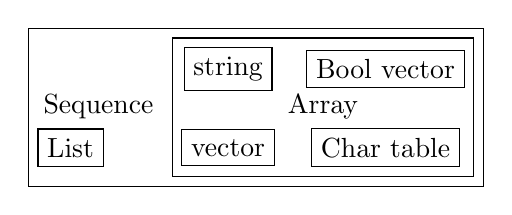
\begin{tikzpicture}
  % \node (A) [rectangle,draw,rounded corners] at (0,1) {hello};
  % \node (B) at (0,2) {yes};
  % \draw (0,1) -- (2,4);
  % \node [rectangle,draw,label=sequence] {
  %   % \node [label=list] {
  %   %   % \node [label="Array"] {};
  %   % };
  % };

  \node (vector) at (0,0) [draw] {vector};
  \node (string) at (0,1) [draw] {string};
  \node (char) at (2,0) [draw] {Char table};
  \node (bool) at (2,1) [draw] {Bool vector};
  \node (array) [draw,fit={(vector) (string) (char) (bool)},"center:Array"] {};
  \node (list) at (-2,0) [draw] {List};
  \node (sequence) [draw,fit={(list) (array)},label={[shift={(-2,0)}]center:Sequence}] {};
\end{tikzpicture}

\begin{description}
\item [length \NT{seq}]
\item [elt \NT{seq idx}] returns the element of \textit{seq} at \textit{index}
\item [copy-sequence \NT{seq}] the sequence is new, but the elements are not.
\end{description}

\subsubsection{array}
It is fixed length sequence.
\begin{description}
% constructing
\item [make-vector \NT{length object}] create vector
\item [vector \NT{\&rest objects}] create vector
% accessing
\item [aref \NT{array index}] getter
\item [aset \NT{array index object}] setter
\end{description}

\subsubsection{hash table}
\begin{description}
% construct
\item [make-hash-table]

% access
\item [gethash \NT{key table}]
\item [puthash \NT{key value table}]
\item [remhash \NT{key table}] remove
\item [clrhash \NT{table}] remove all
\item [maphash \NT{function table}] call function once for each of the
  element in table. The function should accept two arguments: key and
  value
% other
\item [hash-table-count \NT{table}] return number of entries
\end{description}

\subsection{Function}

\begin{description}
  % define
\item [defun \NT{name arglst \&opt docstr decl \&rest body}]
\item [defmacro \NT{name args body}] Macro does not evaluate its
  arguments. It put the arguments /as is/ and put them into the macro
  body to form an expression.  The expression is then evaluated for
  result.

  % Anonymous functions
\item [lambda \NT{args body}]
\item [function \NT{fun-obj}] returns the function without evaluating
  it. It is the "quote" for function
\item [\#'] this is the read syntax for the above \texttt{function}
  special form. You see, it is indeed the \textit{quote} for the
  function.

  % Calling
\item [funcall \NT{fun \&rest args}] compute which function to execute
  at runtime
\item [apply \NT{fun \&rest args}] compute the arguments at
  runtime. Same as =funcall=, but the /last/ of arguments is a list,
  and will be expanded into many arguments instead of a list.

  % Mapping family
\item [mapcar \NT{fun seq}] execute function on each element of
  sequence, and return the list of results.
\item [mapc \NT{fun seq}] same as =mapcar= except it returns the
  =sequence=, with the intention to collect side effect.
\item [mapconcat \NT{fun seq sep}] execute function on
  elements of sequence. The results must be strings, and will be
  concatenated and returned.
\end{description}



\subsection{Control Structure}

\begin{description}
% Sequential
\item [progn \NT{forms...}] return the result of final form
\item [prog1 \NT{form1 forms...}] return the result of form1
\item [prog2 \NT{form1 form2 forms...}] return the result of form2
% Conditional
\item [not]
\item [and]
\item [or]
\item [if \NT{condition then-form else-forms...}]
\item [when \NT{condition then-forms...}]
\item [unless \NT{condition forms...}]
\item [cond \NT{clause...}] the clause must be a list:
  \texttt{(condition body-forms...)}.  It is not exactly the "case"
  statement, because the condition is evaluted to true or false.  Any
  remaining forms are \textit{ignored}.
\item [pcase \NT{exp branch1 branch2 branch3...}] this is more like
  the "case" statement. The EXP is first evaluted and compare with the
  car of each branches.  The branch must be of the form
  \texttt{(UPATTERN BODY-FORMS...)}
\item [while \NT{condition forms...}]
\item [dolist \NT{(var list [result]) body...}] execute body for each
  element of list, with the bound of var to the current element and
  result for return.
\item [dotimes \NT{(var count [result]) body...}] execute body for
  each index of \texttt{[0,count)}, with var bound to the index, and
  result bound for return.
\end{description}

\subsubsection{CL Loop facility}
The package cl-lib.el ports many common lisp facilities into elisp,
most importantly, the loop facility.  So this section, at least for
now, focus on \texttt{cl-loop}.

\begin{description}
\item [cl-loop \NT{clauses...}] general loop form.
\item [for \NT{var} from \NT{from} to \NT{to} by \NT{step}]
  \textit{from} defaults to 0. \textit{step} must be positive and default to 1;
  inclusive \texttt{[from,to]};
  \texttt{from} can be \texttt{upfrom} and \texttt{downfrom}. I think it is wired to use this;
  \texttt{to} can be \texttt{upto} and \texttt{downto}. This makes more sense;
  \texttt{above} and \texttt{below} can be used, but /exclusive/. e.g. \texttt{for var below 10}
\item [for VAR in LIST by FUNCTION] =FUNCTION= is used to traverse the list, defaults to =cdr=
\item [for VAR on LIST by FUNCTION] =VAR= is bound to the cons cell of the list instead of the element.
\item [for VAR across ARRAY] iterates all elements of array
\item [for VAR ]PR1 then EXPR2= :: this is the most general form.  The
  =VAR= is bound to =EXPR1= initially, and will be set by evaluating
  =EXPR2= in successive iterations.  =EXPR2= can refer the old =VAR=

% iteration clauses
\item [repeat \NT{integer}] repeat the loop how many times
\item [while \NT{condition}] stops the loop when the condition becomes nil
\item [until \NT{condition}]
\item [always \NT{condition}] like while except it returns =nil=, and =finally= clauses are not executed.
\item [never \NT{condition}] counter part for =always=

% accumulation clauses
\item [collect \NT{form}] collect into a list and return the list in the end
\item [append \NT{form}] collect the lists into a list by appending, and return it in the end
\item [concat \NT{form}] for string only
\item [count \NT{form}] count how many times form evaluates to non-nil.
\item [sum \NT{form}] sum all the values
\item [maximize \NT{form}] get the max. If the form is never executed, result is /undefined/
\item [minimize \NT{form}]

% Other clauses
\item [with var = value] set the value one-time at the beginning of
  the loop.  Often used as return variable.  *The spaces around ~=~ is
  essential!*.
\item [if condition clause [else clause]]
\item [when condition clause] same as if
\item [unless condition clause] similar
\item [initially [do] forms...] execute before the loop begins, but
  after the =for= and =with= variable bindings. =do= is optional.
\item [finally [do] forms...] execute after the loop finishes
\item [finally return form] finally return it ...
\item [do forms...] execute as an implicit =progn= in the body
\item [return form] this is often used in =if= or =unless=, because
put it in top level will cause the loop always execute only once.
\end{description}



\subsection{Debugging}
\subsubsection{lisp debugger}
The simplest debugger is called =lisp debugger=.
You can turn on the =debug-or-error= flag,
but I found inserting the =(debug)= command useful.
Simply insert =(debug)= where you want program to suspend, and run it.
You will enter the debugger at that point.
In the debugger buffer, the following commands are available:
\begin{description}
\item [c] continue run program
\item [d] step
\item [e] evaluate an prompt expression
\item [R] like =e=, but also save the result in =*Debugger-record*=
\item [q] quit
\item [v] toggle display of local variables ???
\end{description}
\subsubsection{Edebug}
For this to work, first you need to instrument the code.
You can instrument the defun by =C-u C-M-x=.
Actually this is adding a prefix before =eval-defun=,
which instrument, and then evaluate the defun.

After instrumentation, running the defun will cause the program to stop at the first /stop point/ of the function.
The /stop points/ are
\begin{itemize}
\item before and after each subexpression that is a list
\item after each variable reference
\end{itemize}

\begin{description}
\item [b] set a breakpoint. You can also set the /source breakpoints/, by adding =(edebug)=.
\item [u] unset a breakpoint
\item [x CONDITION] set a conditional breakpoint
\item [B] move point to the next breakpoint
\item [w] move point back to the current stop point
\item [<SPC>] run to next stop point
\item [g] execute until next breakpoint
\item [q] exit
\item [S] stop and wait for Edebug commands
\item [n] evaluate a sexp and stop at stop point
\item [t] /trace/, pause one second at each stop point ...
\item [T] rapid trace. Update the display at each stop point but don't actually pause ...
\item [c] pause one second at each breakpoint
\item [C] rapid continue.
\item [G] run and ignore breakpoints (but you can stop it by =S=)

\item [h] proceed to the stop point near the point ...
\item [f] run one expression
\item [o] step out the containing expression
\item [i] step in
\item [e EXP] evaluate a prompt expression
\item [C-x C-e] evaluate an expression at point
\item [?] show help
\item [r] redisplay the most recent sexp result
\item [d] display the backtrace
\end{description}


%%% Local Variables:
%%% TeX-master: "cheatsheet"
%%% End:

\clearpage
\section{\LaTeX}

\subsection{Installation}
To see what is your tex home: \texttt{kpsewhich -var-value=TEXMFHOME}
It should be something like "~/texmf".  Putting class and style file
into correct path inside that folder will enable global usage of the
class.  check whether it works or not: \texttt{kpsewhich
  sig-alternate-05-2015.cls} Typically you don't need to update
database, but if you want, Command to update the =ls-R= database:
\texttt{texhash} or \texttt{mktexlsr}

\begin{tabular}{@{}ll|ll@{}}
  \verb$\alpha$ & $\alpha$ & \verb$\theta$ & $\theta$ \\
  \verb$\phi$ & $\phi$ & \verb$\varphi$ & $\varphi$ \\
  \verb$\xi$ & $\xi$ & \verb$\mu$& $\mu$\\
  \verb$\pi$ & $\pi$ & \verb$\rho$ & $\rho$\\
  \verb$\sigma$ & $\sigma$ & \verb$\epsilon$ & $\epsilon$\\
  \verb$\partial$ & $\partial$\\
  \hline
  \verb$\quad$ & $\alpha\quad\beta$ & \verb$\qquad$ & $\alpha\qquad\beta$\\
  \hline
  \verb$\cup$ & $\cup$ & \verb$\bigcup$ & $\bigcup$ \\
  \verb$\cap$ & $\cap$ & \verb$\vee$ & $\vee$ \\
  \verb$\wedge$ & $\wedge$ & \verb$\in$ & $\in$ \\
  \verb$\notin$ & $\notin$ & \verb$\neg$ & $\neg$ \\
  \verb$\subset$ & $\subset$ & \verb$\subseteq$ & $\subseteq$\\
  \verb$\supset$ & $\supset$ & \verb$\supseteq$ & $\supseteq$ \\
  \verb$\le$ & $\le$ & \verb$\ge$ & $\ge$\\
  \verb$\neq$ & $\neq$ & \verb$\forall$ & $\forall$\\
  \verb$\exists$ & $\exists$\\
  \hline
  \verb$\leftarrow$ & $\leftarrow$ & \verb$\rightarrow$ & $\rightarrow$\\
  \verb$\Rightarrow$ & $\Rightarrow$ & \verb$\Leftarrow$ & $\Leftarrow$\\
  \verb$\Leftrightarrow$ & $\Leftrightarrow$ & \verb$\longrightarrow$ & $\longrightarrow$\\
  \hline
  \verb$\hat{a}$ & $\hat{a}$ & \verb$\vec{x}$ & $\vec{x}$\\
  \hline
  \verb$\infty$ & $\infty$ & \verb$\propto$ & $\propto$\\
  \verb$\lfloor$ & $\lfloor$ & \verb$\rfloor$ & $\rfloor$\\
  \verb$\lceil$ & $\lceil$ & \verb$\rceil$ & $\rceil$\\
  \verb$\sum$ & $\sum$ & \verb$\int$ & $\int$\\
  \verb$\ldots$ & $ \ldots$ & \verb$\frac{a}{b}$ & $\frac{a}{b}$\\
  \verb$\sqrt{n}$ & $\sqrt{n}$ & \verb$\overline{abc}$ & $\overline{abc}$\\
  \verb$\prod$ & $\prod$ & &  \\
  \hline
  \verb$\checkmark$ & $\checkmark$ & \verb$\times$ & $\times$\\
  \hline
  \verb$\tiny$ & \tiny tiny & \verb$\scriptsize$ & \scriptsize scriptsize\\
  \verb$\footnotesize$ & \footnotesize footnotesize& \verb$\small$ & \small small\\
  \verb$\normalsize$ & \normalsize normalsize& \verb$\large$ & \large large\\
  \verb$\Large$ & \Large Large& \verb$\LARGE$ & \LARGE LARGE\\
  \verb$\huge$ & \huge huge& \verb$\Huge$ & \Huge Huge
\end{tabular}



\subsubsection{General Syntax}

\begin{tabular}{@{}l|l|l@{}}
  \begin{lstlisting}
    \begin{enumerate}
    \item xxx
    \end{enumerate}
  \end{lstlisting} &
\begin{lstlisting}
  \begin{itemize}
  \item like this,
  \end{itemize}
\end{lstlisting}&
\begin{lstlisting}
  \begin{description}
  \item[Word] Definition
  \end{description}
\end{lstlisting}\\
\end{tabular}

\begin{tabular}{@{}l|l@{}}
\begin{lstlisting}
  \begin{table}
    \centering
    \begin{tabular}{l|r}
      Item & Quantity \\\hline
      Widgets & 42 \\
      Gadgets & 13
    \end{tabular}
    \caption{\label{tab:widgets}
      An example table.}
  \end{table}
\end{lstlisting} &
\begin{lstlisting}
  \begin{figure}
    \centering
    \includegraphics[width=0.3\textwidth]{frog.jpg}
    \caption{\label{fig:frog}caption.}
  \end{figure}
\end{lstlisting}
\end{tabular}

\begin{tabular}{@{}l|l@{}}
  \begin{lstlisting}
    \label{xxx}
    \ref{xxx}
    \label{xx:yy}
    \ref{xx:yy}
  \end{lstlisting}&
\begin{lstlisting}
\todo{comment in the margin!}
\todo[inline, color=green!40]{inline comment.}
\end{lstlisting}
\end{tabular}

\subsection{Special characters}
\begin{description}
\item [\textbackslash textbackslash] \textbackslash
\item [\textbackslash textasciitilde] \textasciitilde
\end{description}




\subsection{Package: listings}
Predefined languages:
Ada, Algol, Ant, Assembler, Awk, bash, Basic, C, C++, CIL, csh,
Delphi, Eiffel, erlang, Fortran, Gnuplot, Haskell, HTML, Java, Lisp,
LLVM, Lua, make, Matlab, Mercury, ML, Octave, Pascal, Perl, PHP,
PostScript, Prolog, Python, R, Ruby, S, Scala, sh, SQL, tcl, TeX,
VBScript, Verilog, VHDL, XML, XSLT


To make the code listing more pretty, the font needs to be changed.
\verb$\usepackage{courier}$.

global setting:

\begin{lstlisting}
\lstset{basicstyle=\ttfamily,breaklines=true}
% \lstset{frame=b}
\lstset{float,floatplacement=H,captionpos=b}
% \lstset{numbers=left}
\lstset{language=C}
\lstset{showstringspaces=false}
% \lstset{framextopmargin=10pt}
% \lstset{framextopmargin=50pt,frame=t}
% \lstset{float=htb,language=C,frame=single, basicstyle=\small, stringstyle=\ttfamily}
\lstset{escapeinside={(*@}{@*)}}
\end{lstlisting}

\subsection{Package: ulem}

\begin{description}
\item [\textbackslash sout] strike through
\end{description}


\subsection{Package: multicol}
\begin{lstlisting}
\usepackage{multicol}
\begin{multicols}{3}
\end{multicols}
\end{lstlisting}

\subsection{Package: enumitem}
\begin{lstlisting}
\usepackage{enumitem}
\setlist[description]{nosep,style=sameline,leftmargin=3cm,font=\ttfamily}
\setlist[itemize]{nosep,leftmargin=*}
\setlist[enumerate]{nosep}
\end{lstlisting}


%%% Local Variables:
%%% TeX-master: "cheatsheet"
%%% End:

\clearpage
\section{TikZ}

Use of tikz packages.

\begin{lstlisting}
\usepackage{tikz}
\usetikzlibrary{shapes.multipart}
\end{lstlisting}

You can generate picture as pdf file.  To generate figure, add the
following lines, and execute: \texttt{pdflatex -shell-escape
  helium.tex}

\begin{lstlisting}
\usetikzlibrary{external}
\tikzexternalize
\tikzset{external/force remake}
\end{lstlisting}

There's also some library not supported. They need luatex.
\begin{lstlisting}
\usetikzlibrary{graphs,graphdrawing}
\usegdlibrary{layered}
\end{lstlisting}

To create a tikz picture, use
\begin{lstlisting}
  \begin{figure*}[ht]
    \centering
    \begin{tikzpicture}[options]
    \end{tikzpicture}
    \caption{\label{}}
  \end{figure*}
\end{lstlisting}

You can also create picture using \verb$\tikz$ command. It is the
same as begin and end tikzpicture, and put command inside. If only one
command, the curly braces are not required.
\begin{lstlisting}
\tikz[⟨options⟩]{⟨path commands⟩}
\end{lstlisting}

scope can be useful to specify styles.
\begin{lstlisting}
\begin{scope}[color=red]
\end{scope}
\end{lstlisting}

The most common errors for tikz are: miss semicolon; miss curly
braces; miss include tikz library.

Set options by \verb$\tikzset$.
\begin{lstlisting}
\tikzset{>=latex}
\tikzset{grid/.style={gray,very thin,opacity=1}}
\tikzset{anchor/.append code=\let\tikz@auto@anchor\relax}
\tikzset{label anchor/.style={tikz@label@post/.append
    style={anchor=#1}}}
\end{lstlisting}

\subsection{Coordinate}
\begin{lstlisting}
([shift={(2,-0.5)}] iflen.east)
\end{lstlisting}

Inside a path, the first one must be a coordinate. The following ones
can use \texttt{+} or \texttt{++}, meaning shift from current, as well
as shift and move current.

The general syntax is
\begin{lstlisting}
  (<coordinate system> cs:<list of key=value>)
\end{lstlisting}

The following coordinate systems are available:
\begin{description}
\item [canvas]
  \begin{description}
  \item [x]
  \item [y]
  \end{description}
\item [xyz]
  \begin{description}
  \item [x]
  \item [y]
  \item [z]
  \end{description}
\item [canvas polar]
  \begin{description}
  \item [angle]
  \item [radius]
  \item [x radius]
  \item [y radius]
  \end{description}
\item [xyz polar] same as above
  % \begin{description}
  % \item [angle]
  % \item [radius]
  % \item [x radius]
  % \item [y radius]
  % \end{description}
\item [xy polar] alias for \texttt{xyz polar}
\item [node]
  \begin{description}
  \item [name]
  \item [anchor] north, etc
  \item [angle] degreee, e.g. 90, -70
  \end{description}
\item [tangent]
  \begin{description}
  \item [node]
  \item [point]
  \item [solution]
  \end{description}
\end{description}

Using \texttt{calc} library, you can compute the coordinate.
\begin{lstlisting}
([⟨options⟩]$⟨coordinate computation⟩$)
($(a)+3*(1cm,0)$)
\end{lstlisting}



\subsection{Style}
style can be defined.
\begin{lstlisting}
  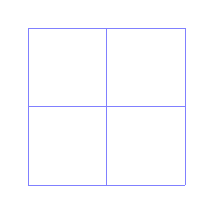
\begin{tikzpicture}[help lines/.style={blue!50,very thin}]
    \draw[help lines] (2,0) grid +(2,2);
  \end{tikzpicture}
\end{lstlisting}

\subsection{Path}
Add \texttt{-- cycle} at the end of a path will complete the path by
connecting back to the start.

\texttt{/tikz/every path} can be used to customize all path.

Operations
\begin{description}
\item [move-to] just coordinates
\item [line-to]
  \begin{description}
  \item [straight line] \texttt{-- (1,1)}
  \item [horizontal and vertical] \texttt{|-} or \texttt{-|}
  \end{description}
\item [curve-to] \texttt{.. controls <c> (and <d>) ..}
\item [rectangle] \texttt{(0,0) rectangle (1,1)}
\item [rounded corners]
\item [sharp corners]
\item [circle] \texttt{circle[⟨options⟩]}. It has option
  \texttt{/tikz/every circle}
  \begin{description}
  \item [x radius]
  \item [y radius]
  \item [radius]
  \item [at]
  \end{description}
\item [ellipse] ellipse[⟨options⟩] Same as circle
\item [arc]
  \begin{description}
  \item [start angle]
  \item [end angle]
  \item [delta angle]
  \end{description}
\item [grid] \verb$\draw[grid] (-2,0) grid (2,12);$
  \begin{description}
  \item [step]
  \item [xstep]
  \item [ystep]
  \item [help lines]
  \end{description}
\item [to] TODO
\item [foreach] TODO
\item [let] TODO
\end{description}

\subsection{Action}
\verb$\draw$ equals \verb$\path{draw}$
Action
\begin{description}
\item [draw]
\item [fill]
\item [filldraw]
\item [pattern] options: \texttt{pattern color}
  \begin{description}
  \item [dots]
  \item [fivepointed stars]
  \item [bricks]
  \end{description}
\item [shade] It has an option \texttt{shading
    angle=<degrees>}. Another option \texttt{shading=<name>} can be:
  \begin{description}
  \item [axis]
  \item [radial]
  \item [ball]
  \end{description}
\item [shadedraw]
\item [clip]
\item [useasboundingbox]
\end{description}


Graphic parameters
\begin{description}
\item [color] used for fill, draw, text. Can use \texttt{red!20!black}
  thanks to \texttt{color} package.
  \begin{description}
  \item [draw=<color>]
  \item [fill=<color>]
  \item [text=<color>] apply on text
  \end{description}

\item [draw] 
\item [line width] Line can be: ultra thin, very thin, thin,
  semithick, thick, very thick, ultra thick. Of course the more
  flexible way is using \texttt{line width = <dimension>}.
\item [dash patterns]
  \begin{description}
  \item [dash pattern=]
  \item [dash phase=]
  \item [solid]
  \item [<densely> <loosely> dotted]
  \item [<densely> <loosely> dashed]
  \item [<densely> <loosely> dash dot]
  \item [<densely> <loosely> dash dot dot]
  \end{description}
\item [double] with option \texttt{double distance=<dimension>}
\end{description}

\subsection{Arrows}
To add the arrow tips, first add \texttt{[->]} option for the tikz
environment.  The library \texttt{arrows.meta} defines etras arrow
types.


\subsection{Node \& Edge}

\begin{lstlisting}
node [⟨options⟩] (⟨name⟩) at (⟨coordinate⟩) {⟨contents⟩};
\end{lstlisting}

\verb$\path node$ equals \verb$\node$. \texttt{every node} and
\texttt{every <shape> node} is available.

Multi part node:
\begin{lstlisting}
  \node[circle split,draw,double,fill=red!20] {top \nodepart{lower} bot};
\end{lstlisting}

\subsubsection{Option}
\begin{description}
\item [align=left] have to have this to make the \verb$\\$ able to create
  newline
\item [shape=<shape name>] \texttt{shape=} is optional. Can be
  rectangle, circle.
\item [inner sep=<dimension>]
\item [inner xsep]
\item [inner ysep]
\item [outer sep]
\item [outer xsep]
\item [outer ysep]
\item [minimum height]
\item [minimum width]
\item [minimum size]
\end{description}


\subsubsection{Position}
\begin{description}
\item [anchor]
\item [above=<offset]
\item [below]
\item [left]
\item [right]
\item [above left]
\item [above right]
\item [below left]
\item [below right]
\item [centered]
\item [fit] \texttt{fit=(a) (b) (c)}
\end{description}

Placing node on edge
\begin{description}
\item [pos=<fraction>]
\item [auto]
\item [swap]
\item ['] alias of swap
\item [sloped]
\item [allow upside down]
\item [midway]
\item [near start] 0.25
\item [near end] 0.75
\item [very near start] 0.125
\item [very near end] 0.875
\item [at start]
\item [at end]
\end{description}

\subsubsection{Label \& Pin}
General syntax is \texttt{label=[<options>]<angle>:<text>}.
\texttt{every label/.style} is available.

Options:
\begin{description}
\item [label position=<angle>]
\item [absolute=boolean]
\item [label distance]
\end{description}

General syntax for pin is \texttt{pin=[<options>]<angle>:<text>}

options:
\begin{description}
\item [pin distance]
\item [every pin]
\item [pin position=<angle>]
\item [every pin edge]
\end{description}

The \texttt{quotes} package provides quote syntax:
\texttt{"<text>"<options>}. The option \texttt{every label quotes} is
available.
\begin{lstlisting}
\tikz \node ["my label" red, draw] {my node};
\end{lstlisting}


\subsection{Graph}
This requires the \texttt{graphs} library.

\begin{description}
\item [graph syntax] \verb$\path graph[⟨options⟩]⟨group specification⟩$
\item [group spec] \verb${[⟨options⟩]⟨list of chain specifications⟩}$
  The nodes can be grouped by surround them with curly braces. The
  entry and exit points are computed for the chains in and out the
  group.

\item [chain spec] consists of list of node spec seperated by edge
  spec
\item [edge spec] each accept an optional \texttt{[<options>]} after them.
  \begin{description}
  \item [->] directed edge
  \item [--] undirected edge
  \item [<-] backward
  \item [<->] bidirected
  \item [-!-] no edge
  \end{description}
\item [node spec] \verb$"<node name>"/"<text>"[<options>]$ The nodes
  used have a special notation. The quotes are required only when the
  node name contains special symbols. If the node name is empty, it
  will be given a random name.
\end{description}

Options
\begin{description}
\item [grow up/down/left/right]
\item [branch up/down/left/right]
\item [grow up/down/right/left sep=<distance>]
\item [branch up/down/left/right sep=<distance>]
\item [/tikz/graph/level <level>] \texttt{level 1/.style={}}
\end{description}

\subsection{Matrix}
The columns are separated by \verb$&$, rows by \verb$\\$. The last
line also needs an \verb$\\$.
\verb$\matrix$ equals to \verb$\path \node [matrix]$
\begin{lstlisting}
  \matrix {
    \node(a) {A}; & \node (b) {B}; \\
    \node(c) {C}; & \node (d) {D}; \\
  };
\end{lstlisting}

options
\begin{description}
\item [column sep]
\item [row sep]
\end{description}

option group
\begin{description}
\item [row/column <number>]
\item [row <number> column <number>]
\item [every odd/even row/column]
\end{description}


\subsection{Tree}

\begin{lstlisting}
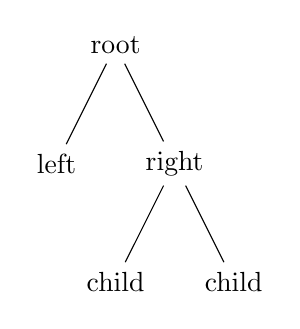
\begin{tikzpicture}
  \node {root}
    child {node {left}}
    child {node {right}
      child {node {child}}
      child {node {child}}
    };
\end{tikzpicture}
\end{lstlisting}

option
\begin{description}
\item [level distance]
\item [grow=<direction>]
\item [grow'=<direction>]
\end{description}

option group
\begin{description}
\item [level <number>]
\end{description}

\subsection{Decoration}
Must have \texttt{decorate} option, then specify the pattern by
\texttt{decoration=}. \texttt{random steps} is useful.

\begin{lstlisting}
decorate, decoration={random steps,segment length=3pt,amplitude=1pt}
\end{lstlisting}


\subsection{Package}
\subsubsection{shapes.multipart}
\begin{lstlisting}
mynode/.style={split, rectangle split parts=2}
\end{lstlisting}
\begin{description}
\item [patterns]
\item [positioning,fit,calc]
\item [decorations.pathmorphing]
\item [decorations.pathreplacing]
\item [quotes]
\item [graphs]
\item [arrows.meta]
\end{description}





%%% Local Variables:
%%% TeX-master: "cheatsheet"
%%% End:

\clearpage
\section{Prolog}

online resources
\begin{itemize}
\item learn prolog now \footnote{http://lpn.swi-prolog.org/lpnpage.php?pageid=top}
\item swipl library \footnote{http://www.swi-prolog.org/pldoc/man?section=lists}
\end{itemize}

\subsection{Running program}

Install swi-prolog, and emacs should be able to support it.  In a
prolog file, select a region, and \texttt{C-c C-c r} (execute region).
Using this for facts and rules, but evalute query direct in the repl.

\subsection{Concepts}

A Horn Clause: $c \quad h_1 \wedge h_2 \wedge \ldots \wedge h_n$.
$c$ is the consequent, the conjunction of $h_i$ is the antecedent.
It means if all $h_i$ are true, $c$ is true.
This is written in prolog as:

\begin{lstlisting}
  c :- h1,h2,...,hn
\end{lstlisting}

Logic program is actually a collection of Horn Clauses.
A logic problem has three components:
\begin{description}
\item [fact] Horn Clause with no Antecedent. isamother(mary)
\item [rule] Horn Clause with Antecendent
\item [query] Horn Clause with no Consequent
\end{description}

Example:

\begin{lstlisting}[language=prolog]
  % facts
  isamother(mary).
  childof(tom, mary).
  % rules
  loves(mary, tom) :- isamother(mary), childof(tom, mary).
  % quries
  ?- loves(mary, tom).
\end{lstlisting}

Prolog can have variables. Everything start from upper case letter or
underscore is a variable. A single underscore is anonymous
variable. Variables are often used in rules and quries.
\begin{lstlisting}
  loves(X, Y) :- isamother(X), childof(Y, X).
  ?- loves(mary, X).
\end{lstlisting}

Syntax of prolog:
\begin{lstlisting}
  Clause :: Predicate. | Predicate :- PredicateSeq.
  PredicateSeq :: Predicate | Predicate, PredicateSeq
  Predicate :: PredName(TermSeq)
  TermSeq :: Term | Term, TermSeq
  Term :: FunctorName(TermSeq) | Constant | Variable
\end{lstlisting}

\subsection{Executing}
\subsubsection{Unification}
Given two atomic formula (predicates), they can be unified if and only
if they can be made syntactically identical by replacing the variables
in them by some terms. For example, unify \texttt{childof(jane, X)}
and \texttt{childof(jane, mary)}.  \textit{MGU} results from a
substitution that bounds free variables as little as possible

\subsubsection{Substitution}
Substitution maps variables to terms.  Instantiation is the
application of substitution to all variables in a prolog formula,
term. E.g. unify $childof(jane, X)$ and $childof(Y, mary)$ by
$[X \rightarrow mary, Y \rightarrow jane]$

\subsubsection{Unification and Computing with Logic}

Given a query
\begin{itemize}
\item Search the facts and rules to find whether the query unifies
  with any consequent
\item If the search fails, return false (query result)
\item If the search is successful, then
  \begin{itemize}
  \item if the unification occurs with the consequent of a fact,
    return the substitution of the variables (if any)
  \item if the unification occurs with the consequent of a fact,
    return the substitution of the variables (if any)
  \end{itemize}
\end{itemize}

An example:
\begin{lstlisting}
isamother(mary).
childof(tom, mary).
loves(X, Y) :- isamother(X), childof(Y, X).
?- loves(mary, tom).
\end{lstlisting}

\subsubsection{Backtracking}

\begin{itemize}
\item Re-try to unify with some clause other than the fact, and proceed
\item Re-try to unify with some clause other than the fact, and proceed
\end{itemize}

Example:
\begin{lstlisting}
isamother(mary).
childof(jane, mary).
childof(tom, mary).
loves(X, Y) :- isamother(X), childof(Y, X).
?- loves(mary, X)
\end{lstlisting}

\subsection{Other Prolog Features}
\subsubsection{List}

\begin{itemize}
\item \texttt{[a, b, c]}: a list of 3 elements
\item \texttt{[]}: empty list
\item \texttt{[a, [b, c], [[d, e]], []]}: list can contain different type
\item \texttt{[a|[b, c]]}: head and tail
\end{itemize}

Example:
\begin{lstlisting}
  ?- [1, 2, 3] = [X|Xs].
  % X=1
  % Xs = [2, 3]
  ?- [1, 2, 3] = [X|[Y|Rest]].
  % X=1
  % Y=2
  % Rest = [3]
\end{lstlisting}

\subsubsection{if-then-else}
\begin{lstlisting}
  ?- Z = 3, (Z == 3 -> X = 1, Y = 2; X = 2, Y = 1).
  % Z=3
  % X=1
  % Y=2
\end{lstlisting}

\subsection{Examples}
\begin{lstlisting}
lectures(monday, nolecture).
lectures(tuesday, vp).
lectures(tuesday, se).
lectures(tuesday, ddbms).
lectures(wednessday, ds).
lectures(wednessday, mpl).
lectures(thursday, vp).
lectures(thrusday, se).
lectures(friday, ds).
lectures(friday, mpl).
lectures(saturday, ai).
lectures(saturday, ddbms).
%% ?- lectures(friday, X), write(X),nl.
%% ?- lectures(friday, X), write(X), nl, fail.
\end{lstlisting}

An graph example:
\begin{lstlisting}
edge(a, b).
edge(b, c).
edge(c, a).
reach(X, Y) :- edge(X, Y).
reach(X, Y) :- edge(X, Z), reach(Z, Y).
?- reach(a, c)
\end{lstlisting}



%%% Local Variables:
%%% TeX-master: "cheatsheet"
%%% End:


% \input{clqr-typographic-conventions}
% \clearpage
% \input{clqr-numbers}
% \input{clqr-characters}
% \input{clqr-strings}
% \input{clqr-conses}
% \input{clqr-arrays}
% \input{clqr-sequences}
% \input{clqr-hash-tables}
% \input{clqr-structures}
% \input{clqr-control-structure}
% \input{clqr-clos}
% \input{clqr-conditions-and-errors}
% \input{clqr-types-and-classes}
% \input{clqr-input-output}
% \input{clqr-packages-and-symbols}
% \input{clqr-compiler}
% \input{clqr-external-environment}

%%%%%%%%%%%%%%%%%%%%%%%%%%%%%%%%%%%%%%%%%%%%%%%%%%
%%%%%%%%%%%%%%%%%%%%%%%%%%%%%%%%%%%%%%%%%%%%%%%%%%
%%%%%%%%%%%%%%%%%%%%%%%%%%%%%%%%%%%%%%%%%%%%%%%%%%
%

% (HEBI: Remove index)
% \clearpagebeforeindex % \clearpage dependent on paper size
% %
% \renewcommand{\indexpagestyle}{lispref}
% \renewenvironment{theindex}%
%                  {\begin{list}{}%
%                      {\setlength{\itemindent}{-1em}\setlength{\leftmargin}{1em}}%
%                      \parskip0pt plus .1pt \itemsep0pt%
%                      \raggedright\looseness=-1%
%                  }%
%                  {\end{list}}
% \begin{multicols}{4}
%   %%%%%%%%%%%%%%%%%%%%%%%%%%%%%%%%%%%%%%%%%%%%%%%%%%
%   [\section*{Index}\vspace{-5ex}]
%   %%%%%%%%%%%%%%%%%%%%%%%%%%%%%%%%%%%%%%%%%%%%%%%%%%
%   % Stock \printindex won't do as we want more than two columns.
%   \tiny\sffamily\input{clqr.ind}
% \end{multicols}


%%%%%%%%%%%%%%%%%%%%%%%%%%%%%%%%%%%%%%%%%%%%%%%%%%
% Make (total) page count a multiple of four.
%%%%%%%%%%%%%%%%%%%%%%%%%%%%%%%%%%%%%%%%%%%%%%%%%%
\clearpage
\pagestyle{empty}
\newcount\currentpage 
\currentpage=\value{page} 
\divide\currentpage by 4  
\multiply\currentpage by 4  
\advance\currentpage by -\value{page}
%
\ifnum\the\currentpage=-3 
\rule{0pt}{0pt}\clearpage
\else\ifnum\the\currentpage=-2
\rule{0pt}{0pt}\clearpage\rule{0pt}{0pt}\clearpage 
\else\ifnum\the\currentpage=-1
\rule{0pt}{0pt}\clearpage\rule{0pt}{0pt}\clearpage\rule{0pt}{0pt}\clearpage 
\fi\fi\fi
%
%%%%%%%%%%%%%%%%%%%%%%%%%%%%%%%%%%%%%%%%%%%%%%%%%%
%% Back Cover
%%%%%%%%%%%%%%%%%%%%%%%%%%%%%%%%%%%%%%%%%%%%%%%%%%
\begin{titlepage}
  \advance\evensidemargin by -1.5mm
  \begin{center}
    \renewcommand{\rmdefault}{ptm} %% Always times fonts on title
    \vspace*{20pt}
    \vfill
    \begin{minipage}{\titlepagewidth}
      \begin{center}
        \rmfamily\mdseries\itshape\fontsize{300}{0}\selectfont
        \reflectbox{{\color{backcovergray}cl\/}}\\
      \end{center}
    \end{minipage}
    \vfill
    \vspace*{40.5mm}% Adjust here if text below changes
    \begin{minipage}{\titlepagewidth}
      \hrule
      \vspace{1.5mm}
      \rmfamily\small
      \makebox[\textwidth][l]{\maintitle\
        \hfill
        Revision \input{REVISION}
        [\input{DATE}\hspace{-.65ex}]}
      \makebox[\textwidth][l]{Copyright \copyright\ 2008 - 2014
        \AUTHOR\hfill}
      \makebox[\textwidth][l]{\LaTeX\ source:
        \href{http://clqr.boundp.org}{http://clqr.boundp.org}
        \hfill
        % \raisebox{-1mm}[0mm][0mm]{\includegraphics[origin=c,height=5mm,keepaspectratio,angle=-40]{housefly.eps}}
      }\\[1mm] 
      Permission is granted to copy, distribute and/or modify this
      document under the terms of the GNU Free Documentation License,
      Version 1.2; with no Invariant Sections, no Front-Cover Texts and
      no Back-Cover Texts.\hfill
      \href{http://www.gnu.org/licenses/fdl.html}{http://www.gnu.org/licenses/fdl.html}\\
      \vspace{-1mm}
      \hrule
    \end{minipage}
  \end{center}
\end{titlepage}

\end{document}
% -*-latex-*-

% LocalWords:  ptm lightgray cl lispref theindex pt

%%% Local Variables: 
%%% mode: latex
%%% TeX-master: t
%%% End: 
